%
% Copyright 2017 Markus Borg, Lund University
%
% This work is licensed under a Creative Commons Attribution-ShareAlike 4.0 International License.
% See http://creativecommons.org/licenses/by-sa/4.0/
%
% The dodument is based on a LaTeX template developed by Jean-Philippe Eisenbarth
% https://github.com/jpeisenbarth/SRS-Tex
%
\documentclass{scrreprt}
\usepackage{graphicx}
\usepackage{listings}
\usepackage{underscore}
\usepackage[bookmarks=true]{hyperref}
\usepackage[utf8]{inputenc}
\usepackage[english]{babel}
\hypersetup{
    bookmarks=false,    % show bookmarks bar?
    pdftitle={Lab 2},    % title
    pdfauthor={Markus Borg},                     % author
    pdfsubject={TeX and LaTeX},                        % subject of the document
    pdfkeywords={TeX, LaTeX, graphics, images}, % list of keywords
    colorlinks=true,       % false: boxed links; true: colored links
    linkcolor=blue,       % color of internal links
    citecolor=black,       % color of links to bibliography
    filecolor=black,        % color of file links
    urlcolor=purple,        % color of external links
    linktoc=page            % only page is linked
}%
\def\myversion{0.4 }
\date{}
%\title
\usepackage{hyperref}
\begin{document}

\begin{flushright}
    \rule{16cm}{5pt}\vskip1cm
    \begin{bfseries}
    	\LARGE{ETSA02-ADM-LAB2}\\
    	\vspace{1.5cm}
        \Huge{Lab 2}\\
        \vspace{0.5cm}
        Object-oriented design\\
        \vspace{0.5cm}
        and unit testing\\
        \vspace{1.5cm}
        \LARGE{Version \myversion approved}\\
        \vspace{1.5cm}
        Prepared by Markus Borg\\
        %\vspace{1.5cm}
        Dept. of Computer Science, Lund University\\
        \vspace{1.5cm}
        \today\\
    \end{bfseries}
\end{flushright}

%\tableofcontents

\chapter*{Revision History}

\begin{center}
    \begin{tabular}{|c|c|c|c|}
        \hline
	    Name & Date & Reason For Changes & Version\\
        \hline
	    Markus Borg & 2017-12-11 & Initial draft. & 0.1\\
        \hline
        Markus Borg & 2018-03-21 & Changed to refactoring+unit testing. & 0.2\\
        \hline
        Markus Borg & 2018-03-21 & Complete draft. & 0.3\\
        \hline
        Markus Borg & 2018-03-22 & Updated after internal review. & 0.4\\
        \hline
    \end{tabular}
\end{center}

\chapter{Introduction}
Lab 2 will inspire you to organize your robot implementation according to a a proper object-oriented design. Furthermore, the lab will help you get started with unit testing using the JUnit framework. More specifically, Lab 2 covers:

\begin{itemize}
\item Program comprehension, i.e., reading code of a somewhat more advanced robot.
\item Reading a UML class diagram.
\item Refactoring source code.
\item Working with JUnit in Eclipse.
\end{itemize}

\chapter{Before the lab}
To save time during the lab session, please read through this section and follow the instructions. Also, unless you are already familiar with it, please read how the Robocode coordinate system works. One source to understand navigation in Robocode is this link: http://mark.random-article.com/weber/java/robocode/lesson4.html

Wikipedia is a great source to read up on software engineering topics. Software engineers appear to carefully monitor and describe their work practices. Perhaps they take pride in describing what they do for the masses? Good for us, Wikipedia (at least in English) is a free and accurate source of software engineering knowledge. Besides, reading from other sources than the course book is a good idea.

Prior to the lab, please browse the following Wikipedia articles:
\begin{itemize}
\item Object oriented programming (skip ``History'' and onwards)\\-- https://en.wikipedia.org/wiki/Object-oriented_programming)
\item Class diagram\\-- https://en.wikipedia.org/wiki/Class_diagram
\item Code refactoring\\-- https://en.wikipedia.org/wiki/Code_refactoring
\item Unit testing\\-- https://en.wikipedia.org/wiki/Unit_testing
\end{itemize}

The course material is under development under an open source license on GitHub. Have a look at: https://github.com/lunduniversity/introsofteng
If you are already familiar with git, I strongly recommend that you clone the repository. If you don't know what this means, instead click the button presented in Figure~\ref{fig:github} and choose ``Download ZIP''. Your lab instructor can help you getting started with git, but simply extracting the Lab2 files from the zip archive works fine as well. In Lab 2, you need the files located in introsofteng-master/project/rumble/labs/lab2/src, including its subfolder. Once you are comfortable with git, you are most welcome to create ``pull requests'' to improve the course material, e.g., clarifying descriptions or correcting typos!

\begin{figure}
\centering
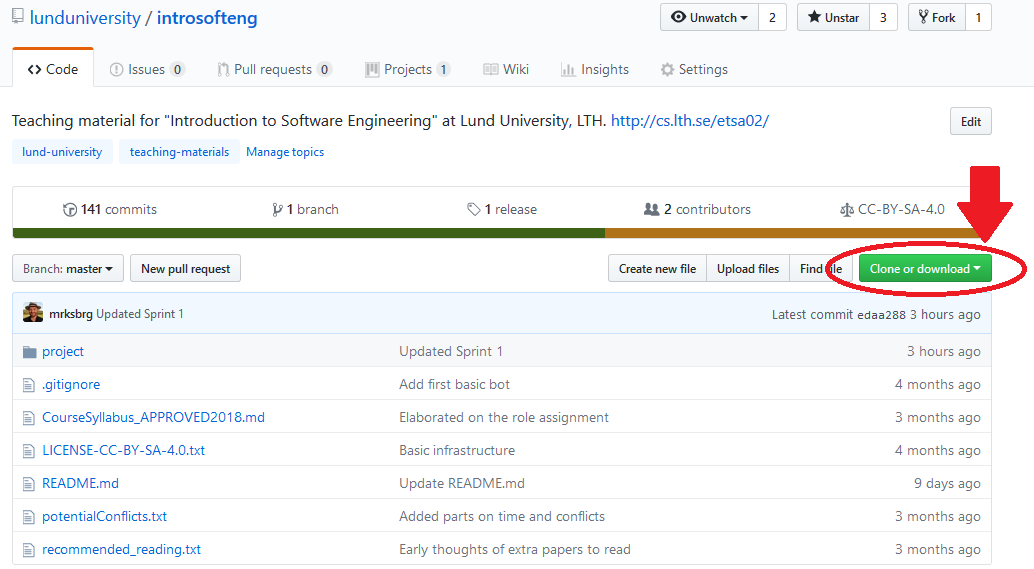
\includegraphics[width=0.99\textwidth]{figures/GitHub.png}
\caption{introsofteng repository on GitHub. The arrow shows the ``Clone or download'' button.}
\label{fig:github}
\end{figure}

\chapter{At the lab}
The first thing you need to do is to get started with automated testing using JUnit. Start by following the following steps:
\begin{enumerate}
\item Create a new Java project in your Eclipse workplace. As in Lab 1, add the robocode.jar as an ``External JAR'' in the Libraries tab, either when creating the project or afterwards in the project properties.
\item In the ``Package Explorer'' pane, right click ``src'' and create a new ``Package'' called ``etsa02_lab''.
\item In the ``Package Explorer'' pane, right click the newly created package and run ``Import...''. Select ``File system'' and select all downloaded files in both the ``src'' folder and the ``src/test'' folder. The content in the Package Explorer should resemble Figure~\ref{fig:afterImport}.
\item To make the etsa02_lab2.test package build, you must configure JUnit. Right click the Java project and select ``Properties''. In the ``Java Build Path'', select the ``Libraries'' tab. You should find robocode.jar, now let's add JUnit! Click ``Add Library...'' and select JUnit. Click ``Next >'' followed by ``Finish'' to accept the defaut settings. You should now see JUnit in the Package Explorer in Eclipse.
\item Right click ``AllBasicMeleeBotUnitTests.java'' and choose ``Run as..'' and create a new JUnit run configuration. Give the configuration a descriptive name, such as ``Lab2 unit tests''.
\item Run the unit tests. All of them are supposed to fail!
\end{enumerate}

\begin{figure}
\centering
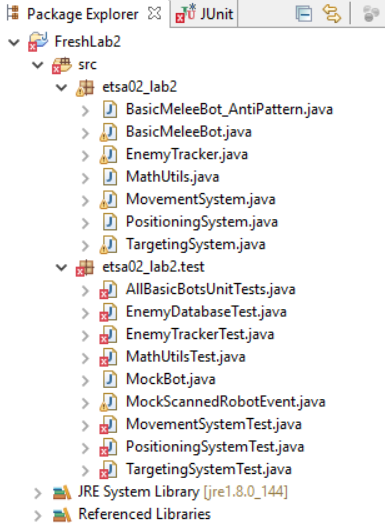
\includegraphics[width=0.5\textwidth]{figures/packageExplorerAfterImport.png}
\caption{The Package Explorer in Eclipse after importing the Lab 2 source code.}
\label{fig:afterImport}
\end{figure}

\newpage

Now it is time to start the refactoring task. 
\begin{enumerate}
\item First, you should study the implementation of the robot in ``BasicMeleeBot_AntiPattern''. The robot implements ``anti gravity movement'', i.e., it moves away from other robots. 
\item Try the robot in Robocode to verify the anti gravity movement.
\item BasicMeleeBot_AntiPattern does not comply with good object oriented design practices, instead all functionality is collected in one big class. A modular robot design would greatly increase the evolvability of the product. Figure~\ref{fig:classDiagram} shows a more feasible object oriented design. Perhaps you can use something similar in your project?
\item Your task is now to refactor BasicMeleeBot_AntiPattern into the structure presented in the provided class diagram. BasicMeleeBot is already implemented for you, but you should complete the missing code in the other classes. A suggested implementation order is: 1) MathUtils, 2) PositioningSystem, 3) EnemyTracker, 4) TargetingSystem, and 5) MovementSystem. The unit tests are there to guide you in the process. Study the test cases to understand the intention behind the different methods. Most importantly, run them frequently to verify that you are on the right track -- when all test cases are green, you have completed Lab 2!
\end{enumerate}

\begin{figure}
\centering
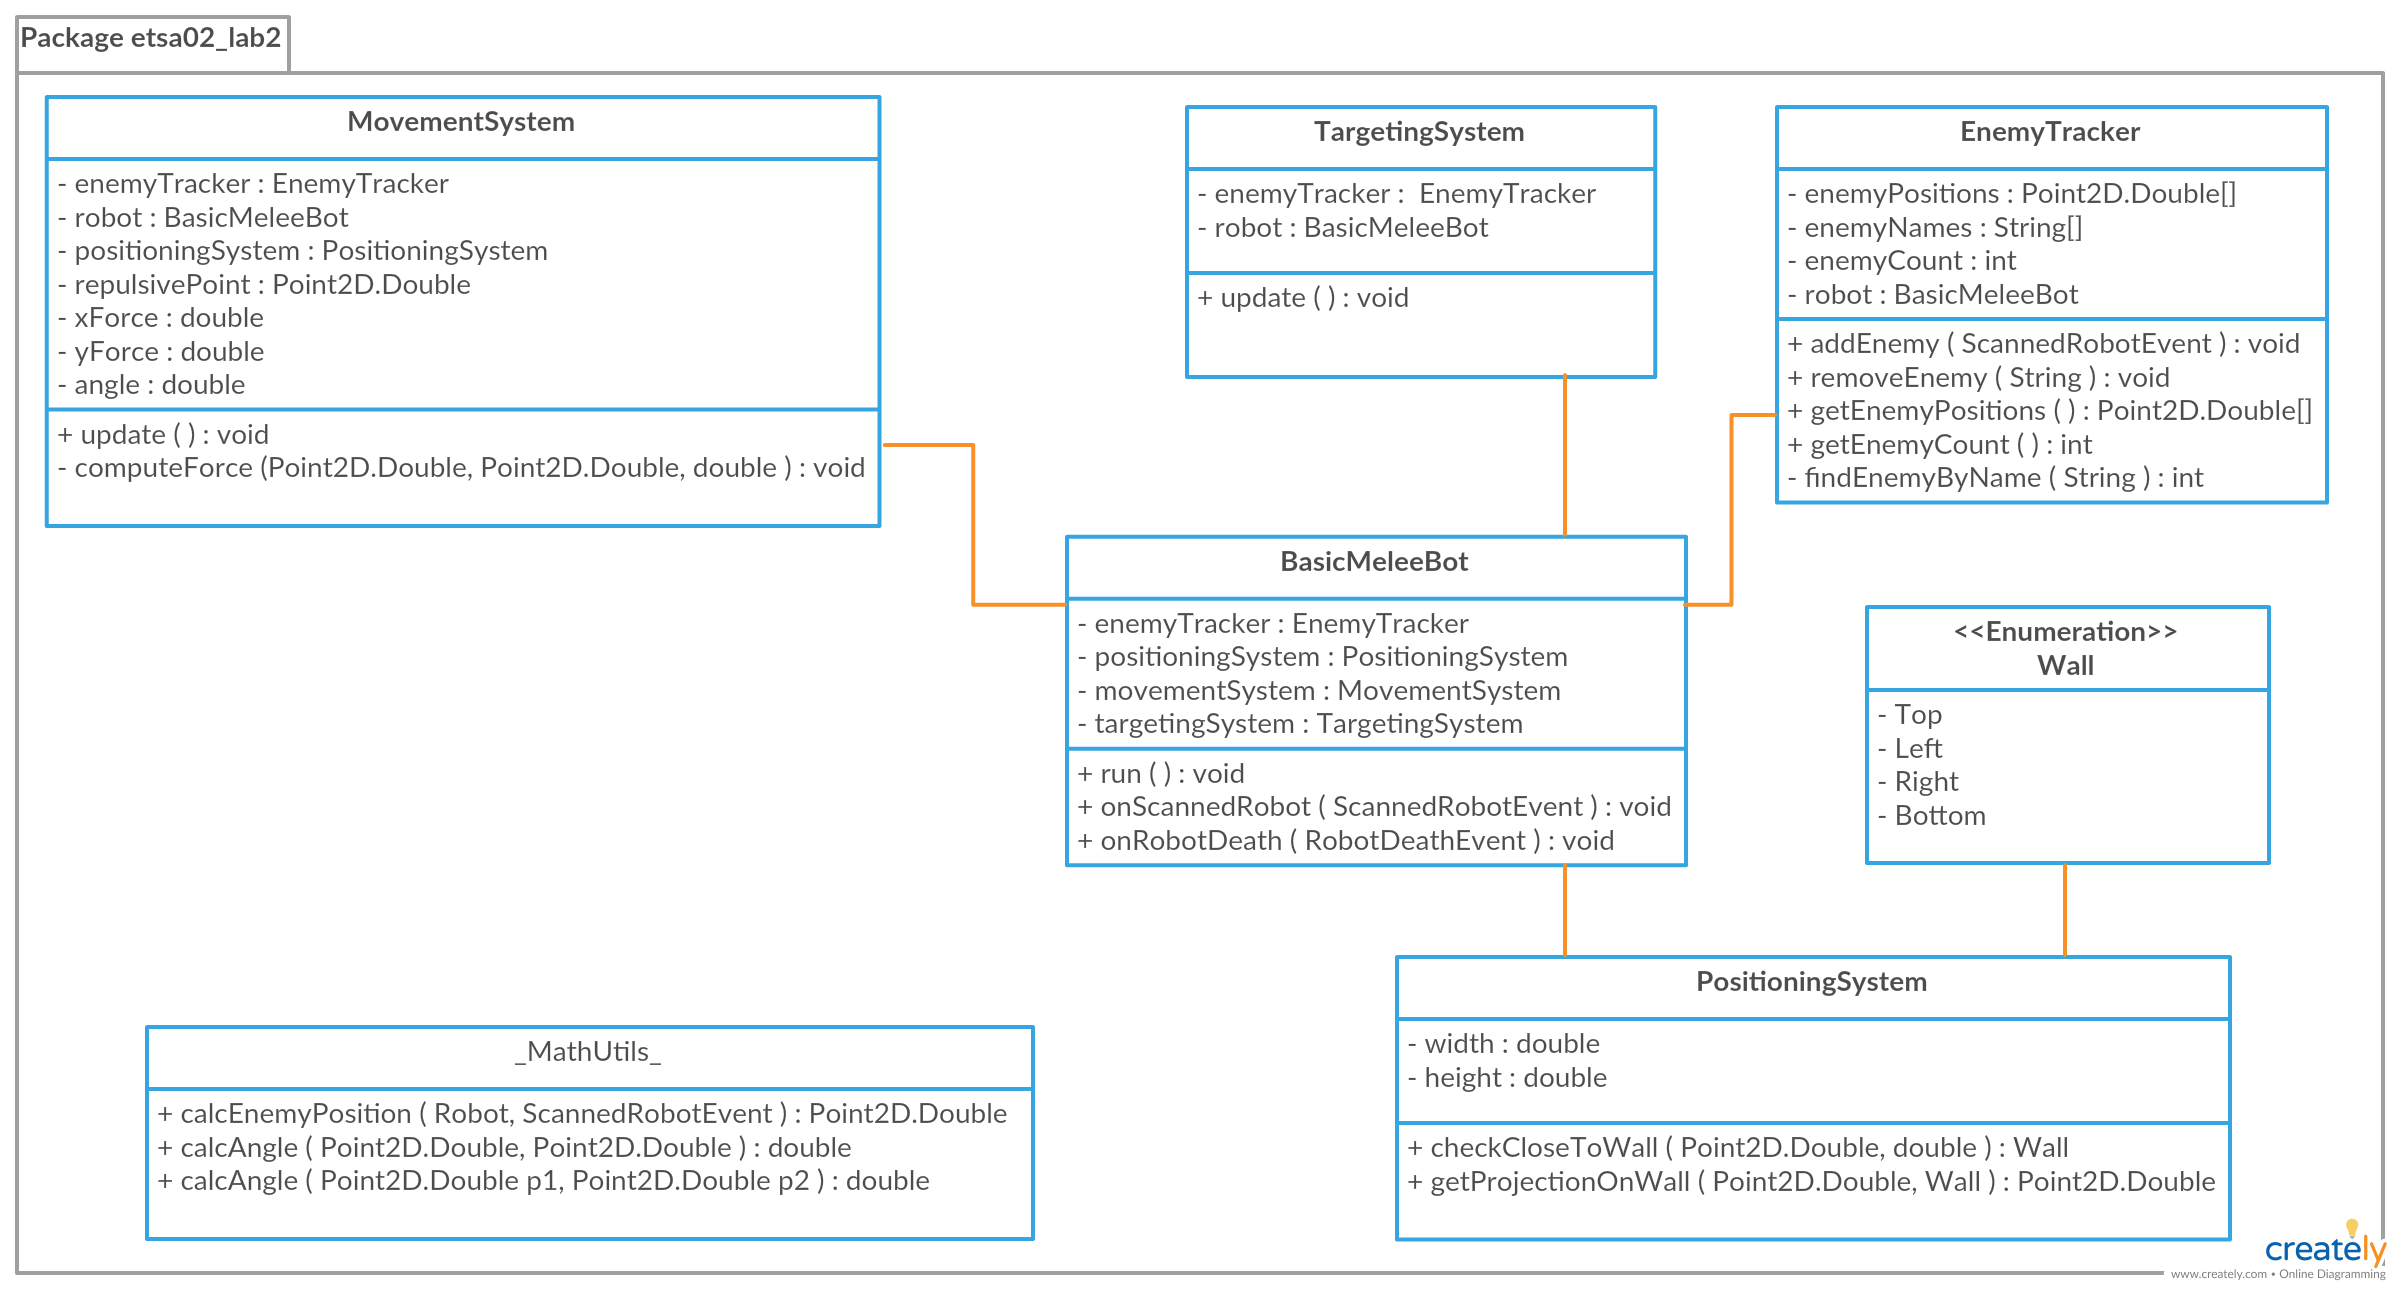
\includegraphics[width=1.1\textwidth]{figures/BasicMeleeBotClassDiagram.png}
\caption{BasicMeleeBot class diagram. Note that MathUtils is a static class.}
\label{fig:classDiagram}
\end{figure}

\newpage

The following instructions are optional, in case you finish the refactoring task quickly. If you complete this task, you will have something similar to the BasicMeleeBot that will be offered as an ETSA02 basic bot on Robot Market. If you don't complete this task during the lab session, you will anyway get the corresponding source code.

Try to improve the behavior of BasicMeleeBot. As you might have noticed, the robot gets stuck in walls when it performs the anti gravity movement. A standard approach to solve this is to implement some form of ``wall avoidance'' strategy. Add wall avoidance to the update() method in the class MovementSystem, and use the methods in PositioningSystem to implement this improvement. Is it possible to add any unit tests for this behavior? If so, add new unit tests to the test suite in MovementSystemTest. If not, try to explain why.

\chapter{After the lab}
During the lab you have practiced several fairly advanced software engineering practices at the same time. You have refactored source code into a modular object-oriented design, guided by a UML class diagram, while adhering to a test-driven development approach supported by automated unit testing. Well done!

When your project releases software, you are supposed to provide the regulatory body with a UML class diagram and source code complemented with a suite of JUnit test cases. Note that the group purchasing your robot should not receive anything of this, they get only the requirements specification, the test specification, and the actual robot as a .jar file.

We recommended that the group helps the development lead to maintain a class diagram of the most recent robot design. Also, the group should help the test lead to evolve a JUnit test suite as an approach to detect bugs early -- you should obviously run your test suite frequently. In industry, the developers are typically responsible for writing unit tests for all their source code, but in the ETSA02 project we expect the test lead to be drive this task. 

\end{document}
